\documentclass[12pt, a4paper]{article}

% Text languages
\usepackage[spanish, english, UKenglish, USenglish, american, british]{babel}

% Accents
\usepackage[latin1]{inputenc}

% Maths
\usepackage{mathtools}
\usepackage{amsmath,amsthm,amssymb}

% Double rows
\usepackage{multirow}

% Math-mode symbol & verbatim
\def\W#1#2{$#1{#2}$ &\tt\string#1\string{#2\string}}
\def\X#1{$#1$ &\tt\string#1}
\def\Y#1{$\big#1$ &\tt\string#1}
\def\Z#1{\tt\string#1}

% A non-floating table environment.
\makeatletter
\renewenvironment{table}%
   {\vskip\intextsep\parskip\z@
    \vbox\bgroup\centering\def\@captype{table}}%
   {\egroup\vskip\intextsep}
\makeatother

\DeclarePairedDelimiter\abs{\lvert}{\rvert}%
\DeclarePairedDelimiter\norm{\lVert}{\rVert}%

% Swap the definition of \abs* and \norm*, so that \abs
% and \norm resizes the size of the brackets, and the 
% starred version does not.
\makeatletter
\let\oldabs\abs
\def\abs{\@ifstar{\oldabs}{\oldabs*}}
%
\let\oldnorm\norm
\def\norm{\@ifstar{\oldnorm}{\oldnorm*}}
\makeatother

% C++
\usepackage{listings}
\usepackage{xcolor}
\lstset { %
	language = C++,
	backgroundcolor=\color{black!5}, % set backgroundcolor
    basicstyle=\footnotesize,% basic font setting
    tabsize=4, % tab space width
    showstringspaces=false, % don't mark spaces in strings
    %numbers=left, % display line numbers on the left
    commentstyle=\color{green}, % comment color
    keywordstyle=\color{blue}, % keyword color
    stringstyle=\color{red} % string color
}

% https://www.overleaf.com/learn/latex/Page_size_and_margins
\usepackage{geometry}
\topmargin = -23pt
\oddsidemargin = 13pt
\headheight = 12pt
\headsep = 25pt
\textheight = 674pt
\textwidth = 426pt
\marginparsep = 10pt
\marginparwidth = 50pt
\footskip = 30pt
\marginparpush = 5pt
\hoffset = 0pt
\voffset = 0pt
\paperwidth = 597pt
\paperheight = 845pt

% Hyperlinks
\usepackage{hyperref}

% Figure
\usepackage{graphicx}
\usepackage{caption}
\usepackage{subcaption}
\usepackage{etoc}
% Example
\newtheorem{exmp}{Example}[section]
% Algorithms
%\usepackage[]{algorithm2e}
%\usepackage{algorithm}% http://ctan.org/pkg/algorithm
%\usepackage{algpseudocode}% http://ctan.org/pkg/algorithmicx
\usepackage{algpseudocode}

\renewcommand{\thefootnote}{\arabic{footnote}} % 1, 2, 3... (la que hay por defecto)

\usepackage{titlesec}
\setcounter{secnumdepth}{5}

\titleformat{\paragraph}
{\normalfont\normalsize\bfseries}{\theparagraph}{1em}{}
\titlespacing*{\paragraph}
{0pt}{3.25ex plus 1ex minus .2ex}{1.5ex plus .2ex}

\usepackage{float}
%--------------------------------------------------------------------------
\title{PARALLELISM}
\author{Roger Vilaseca Darné and Xavier Martín Ballesteros\\
  \small UNIVERSITAT POLITÈCNICA DE CATALUNYA\\
}
\date{10th December 2018}

\begin{document}
% Images
\graphicspath{ {./lab2/images} }

%\maketitle

\begin{titlepage}
	\centering
	%{\scshape\LARGE UNIVERSITAT POLITÈCNICA DE CATALUNYA \par}
	\vspace{1cm}
	{\scshape\Large UNIVERSITAT POLITECNICA DE CATALUNYA\par}
	\vspace{1.5cm}
	{\huge\bfseries PARALLELISM\par}
	\vspace{2cm}
	{\Large\itshape Roger Vilaseca Darne and Xavier Martin Ballesteros\break PAR4110\par}
	\vfill
	{\Large\itshape \textbf{Lab 2: Brief tutorial on OpenMP programming model}\par}
	\vfill
%	
\includegraphics[width=0.25\textwidth]{./images/UPC.png}\par\vspace{1cm}
	%supervised by\par
	%Dr.~Mark \textsc{Brown}

	\vfill

% Bottom of the page
	{\large 20th March 2019, Q1}
\end{titlepage}

%\abstract{Esto es una plantilla simple para un articulo en \LaTeX.}

%	*********************** ÍNDEX *********************
\setcounter{secnumdepth}{5}
\setcounter{tocdepth}{5}

\newpage
  \tableofcontents
\newpage

\section{Introduction}

% Referència a una equació \ref{eq:area}).
% Referència a una secció \ref{sec:nada}
% Referència a una cita \cite{Cd94}.

\section{OpenMP questionnaire}

\subsection{Parallel regions}

\subsubsection{1.hello.c}

\textbf{1. How many times will you see the "Hello world!" message if the program is executed with
"./1.hello"?}

\hfill

\textbf{2. Without changing the program, how to make it to print 4 times the "Hello World!" message?}

\subsubsection{2.hello.c}

\textbf{1. Is the execution of the program correct? (i.e., prints a sequence of "(Thid) Hello (Thid)
world!" being Thid the thread identifier). If not, add a data sharing clause to make it correct?}

\hfill

\textbf{2. Are the lines always printed in the same order? Why the messages sometimes appear intermixed? (Execute several times in order to see this).}

\subsubsection{3.how many.c}

\textbf{Assuming the OMP NUM THREADS variable is set to 8 with "export OMP NUM THREADS=8"}

\hfill

\textbf{1. How many "Hello world ..." lines are printed on the screen?}

\hfill

\textbf{2. What does omp get num threads return when invoked outside and inside a parallel region?}

\subsubsection{4.data sharing.c}

\textbf{1. Which is the value of variable x after the execution of each parallel region with different datasharing attribute (shared, private, firstprivate and reduction)? Is that the value you
would expect? (Execute several times if necessary)}

\subsection{Loop parallelism}

\subsubsection{1.schedule.c}

\textbf{1. Which iterations of the loops are executed by each thread for each schedule kind?}

\subsubsection{2.nowait.c}

\textbf{1. Which could be a possible sequence of printf when executing the program?}

\hfill

\textbf{2. How does the sequence of printf change if the nowait clause is removed from the first for
directive?}

\hfill

\textbf{3. What would happen if dynamic is changed to static in the schedule in both loops? (keeping
the nowait clause)}

\subsubsection{3.collapse.c}

\textbf{1. Which iterations of the loop are executed by each thread when the collapse clause is used?}

\hfill

\textbf{2. Is the execution correct if the collapse clause is removed? Which clause (different than
collapse) should be added to make it correct?}

\subsection{Synchronization}

\subsubsection{1.datarace.c}

\textbf{(execute several times before answering the questions)}

\hfill

\textbf{1. Is the program always executing correctly?}

\hfill

\textbf{2. Add two alternative directives to make it correct. Explain why they make the execution
correct.}

\subsubsection{2.barrier.c}

\textbf{1. Can you predict the sequence of messages in this program? Do threads exit from the barrier
in any specific order?}

\subsubsection{3.ordered.c}

\textbf{1. Can you explain the order in which the "Outside" and "Inside" messages are printed?}

\hfill

\textbf{2. How can you ensure that a thread always executes two consecutive iterations in order during
the execution of the ordered part of the loop body?}

\subsection{Tasks}

\subsubsection{1.single.c}

\textbf{1. Can you explain why all threads contribute to the execution of instances of the single worksharing construct? Why are those instances appear to be executed in bursts?}

\subsubsection{2.fibtasks.c}

\textbf{1. Why all tasks are created and executed by the same thread? In other words, why the program
is not executing in parallel?}

\hfill

\textbf{2. Modify the code so that the program correctly executes in parallel, returning the same answer
that the sequential execution would return.}

\subsubsection{3.synchtasks.c}

\textbf{1. Draw the task dependence graph that is specified in this program}

The \textbf{depend} clause establish dependences, only between tasks, on the scheduling of tasks. There are different types of dependence:

\begin{itemize}
	\item \textbf{in}: The task has to wait until all previously generated sibling tasks that reference at least one of the list items in an \textit{out} or \textit{inout} list end their execution.
	\item \textbf{out} and \textbf{inout}: The task has to wait untill all previously generated sibling tasks that reference at least one of the list items in an \textit{in}, \textit{out} or \textit{inout} list end their execution.
\end{itemize}

In the given code, the first task has an \textbf{out} depende type, with only the variable \textit{a} in its list. As there are no previously generated sibling tasks, this first task is not dependent of any task. Tasks 2 and 3 are not dependent of any previously generated sibling task. Although there exist some previously sibling tasks, none of them has variables \textit{b} or \textit{c} in its lists.

On the other hand, task 4 has an \textbf{in} dependence type with variables \textit{a} and \textit{b} and an \textbf{out} dependence type with variable \textit{d}. Thus, this task will have to wait until tasks 1 and 2 end their execution.

Finally, task 5 has an \textbf{in} dependence type with variables \textit{c} and \textit{d}. This taks will depend from tasks 3 and 4. Hence, the task dependence graph is the following:

\begin{figure}[H]
  \centering
  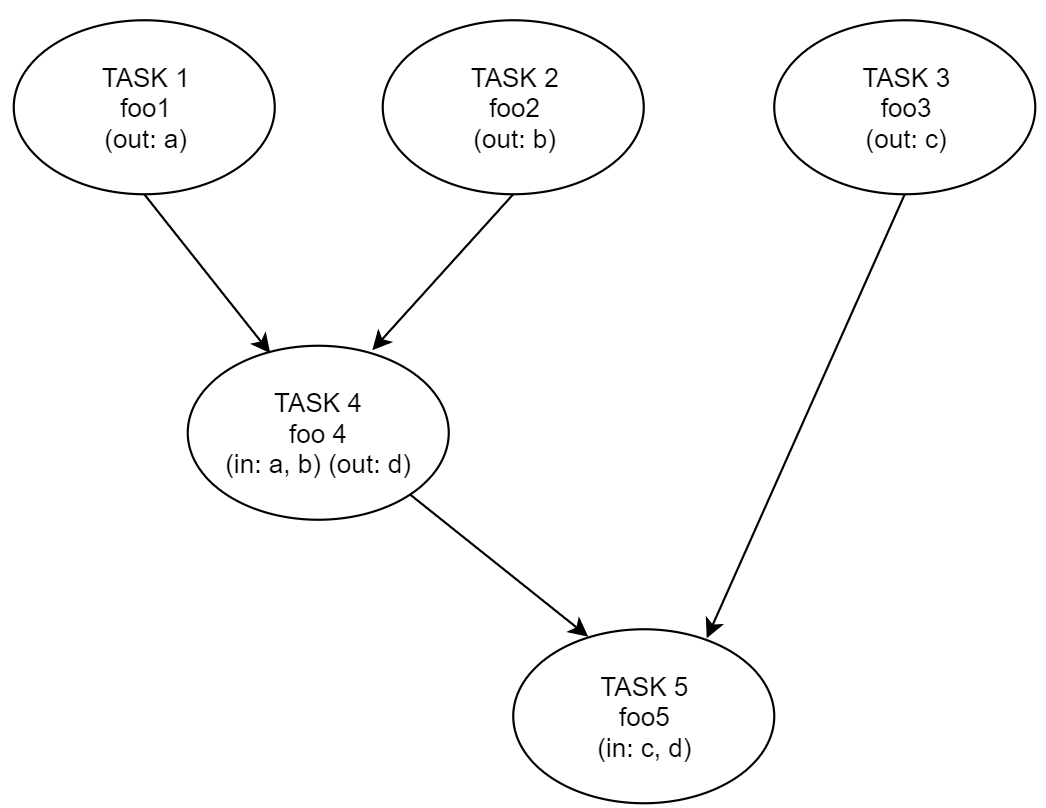
\includegraphics[scale=0.5]{./images/synchtasks}
  \caption{Task dependency graph of code 3.synchtasks.c.}
  \label{Task dependency graph of code 3.synchtasks.c.}
\end{figure}

\hfill

\textbf{2. Rewrite the program using only taskwait as task synchronisation mechanism (no depend clauses allowed)}

The \textbf{taskwait} construct makes a task wait until the completion of its child tasks. The new version of the code is shown below. Task 4 will wait until tasks 1 and 2 end their execution and task 5 will wait until the completition of tasks 3 and 4. Doing this we recreated the task dependency graph of Figure \ref{Task dependency graph of code 3.synchtasks.c.} without using the \textbf{depend} clause.

The first problem we have seen is that task 3 cannot be executed at the same time than tasks 1 and 2. Otherwise, task 4 would have to wait until tasks 1, 2 and 3 end their execution altough it does not depend from task 3. The second problem is that with this code, we are not able to create the 5 tasks at the same time. Tasks 1, 2 and 4 will be created first. Then tasks 3 and 5.

\begin{figure}[H]
	\begin{lstlisting}
	printf("Creating task foo1\n");
	#pragma omp task
	foo1();
	
	printf("Creating task foo2\n");
	#pragma omp task
	foo2();
	
	printf("Creating task foo4\n");
	#pragma omp taskwait
	foo4();

	printf("Creating task foo3\n");
	#pragma omp task
	foo3();
	
	printf("Creating task foo5\n");
	#pragma omp taskwait
	foo5();
	\end{lstlisting}
	
	\caption{Modified version of the given code.}
\end{figure}

Figures \ref{fig:original_code} and \ref{fig:modified_code} show the output when executing the two versions of the code. We can see clearly the differences between one and the other explained before.

\begin{figure}[H]
\begin{minipage}[b]{0.47\linewidth}

\begin{lstlisting}
	Creating task foo1
	Creating task foo2
	Creating task foo3
	Creating task foo4
	Creating task foo5
	Starting function foo3
	Starting function foo1
	Starting function foo2
	Terminating function foo1
	Terminating function foo2
	Starting function foo4
	Terminating function foo4
	Terminating function foo3
	Starting function foo5
	Terminating function foo5
\end{lstlisting}

\caption{Output of the original version of the code.}
\label{fig:original_code}
\end{minipage}
\hspace{0.5cm}
\begin{minipage}[b]{0.48\linewidth}

\begin{lstlisting}
	Creating task foo1
	Creating task foo2
	Creating task foo4
	Starting function foo2
	Starting function foo1
	Terminating function foo2
	Terminating function foo1
	Starting function foo4
	Terminating function foo4
	Creating task foo3
	Creating task foo5
	Starting function foo3
	Terminating function foo3
	Starting function foo5
	Terminating function foo5
\end{lstlisting}

\caption{Output of the modified version of the code.}
\label{fig:modified_code}
\end{minipage}
\end{figure}

\subsubsection{4.taskloop.c}

\textbf{1. Find out how many tasks and how many iterations each task execute when using the grainsize and num tasks clause in a taskloop. You will probably have to execute the program several times in order to have a clear answer to this question.}

The \textbf{grainsize(grain-size)} clause controls how many loop iterations are assigned to each created task. The number of loop iterations assigned to each created task is greater than or equal to the minimum of the value of grain-size and the total number of iterations.

We though that when using the \textbf{grainsize(5)} clause there will be created 3 tasks, the first two executing 5 iterations and the other one 2. In reality, there are only 2 tasks created, each one executing 6 iterations. This is because the number 5 does not mean that each task has 5 iterations but a minimum of 5, unless there remain less than 5 iterations.

The \textbf{num\_tasks(num-tasks)} clause creates as many tasks as the minimum of num-tasks and the number of loop iterations.

There are 5 tasks created. The first two execute 3 iterations of the loop whereas the other 3 execute only 2.

\begin{figure}[H]
	\begin{lstlisting}
	Going to distribute 12 iterations with grainsize(5) ...
	Loop 1: (1) gets iteration 0
	Loop 1: (1) gets iteration 1
	Loop 1: (1) gets iteration 2
	Loop 1: (1) gets iteration 3
	Loop 1: (2) gets iteration 6
	Loop 1: (2) gets iteration 7
	Loop 1: (2) gets iteration 8
	Loop 1: (2) gets iteration 9
	Loop 1: (2) gets iteration 10
	Loop 1: (2) gets iteration 11
	Loop 1: (1) gets iteration 4
	Loop 1: (1) gets iteration 5
	Going to distribute 12 iterations with num_tasks(5) ...
	Loop 2: (2) gets iteration 0
	Loop 2: (2) gets iteration 1
	Loop 2: (1) gets iteration 6
	Loop 2: (1) gets iteration 7
	Loop 2: (0) gets iteration 10
	Loop 2: (0) gets iteration 11
	Loop 2: (1) gets iteration 8
	Loop 2: (1) gets iteration 9
	Loop 2: (2) gets iteration 2
	Loop 2: (3) gets iteration 3
	Loop 2: (3) gets iteration 4
	Loop 2: (3) gets iteration 5
	\end{lstlisting}
	
	\caption{Ouput of the code without the nogroup clause.}
\end{figure}

\hfill

\textbf{2. What does occur if the nogroup clause in the first taskloop is uncommented?}

The \textbf{taskloop} clause implicitly generates a \textbf{taskgroup} region that encloses it. In this region there is a barrier at the end, so the second loop will not be executed until the first one terminates. The \textbf{nogroup} clause removes the \textbf{taskgroup} region.

With the \textbf{nogroup} clause, the second loop can be executed at the same time than the first loop.

Now, there are created the same number of tasks, and each one does the same itreations than in the previous question. However, while two threads execute the first loop, the other two threads will execute the 5 tasks of the second loop (Figure \ref{Ouput 1 of the code with the nogroup clause.}), unless one of the two threads of the first loop end before the second loop terminates. In this situation, this thread will also execute tasks of the second loop (Figure \ref{Ouput 2 of the code with the nogroup clause.}).

\begin{figure}[H]
	\begin{lstlisting}
	Going to distribute 12 iterations with grainsize(5) ...
	Going to distribute 12 iterations with num_tasks(5) ...
	Loop 1: (1) gets iteration 0
	Loop 1: (1) gets iteration 1
	Loop 1: (2) gets iteration 6
	Loop 1: (2) gets iteration 7
	Loop 1: (2) gets iteration 8
	Loop 1: (1) gets iteration 2
	Loop 2: (0) gets iteration 10
	Loop 2: (0) gets iteration 11
	Loop 2: (0) gets iteration 8
	Loop 2: (3) gets iteration 0
	Loop 2: (3) gets iteration 1
	Loop 2: (3) gets iteration 2
	Loop 2: (3) gets iteration 3
	Loop 2: (3) gets iteration 4
	Loop 2: (3) gets iteration 5
	Loop 2: (3) gets iteration 6
	Loop 2: (3) gets iteration 7
	Loop 1: (1) gets iteration 3
	Loop 1: (1) gets iteration 4
	Loop 1: (1) gets iteration 5
	Loop 2: (0) gets iteration 9
	Loop 1: (2) gets iteration 9
	Loop 1: (2) gets iteration 10
	Loop 1: (2) gets iteration 11
	\end{lstlisting}
	
	\caption{Ouput 1 of the code with the nogroup clause.}
	\label{Ouput 1 of the code with the nogroup clause.}
\end{figure}

\begin{figure}[H]
	\begin{lstlisting}
	Going to distribute 12 iterations with grainsize(5) ...
	Going to distribute 12 iterations with num_tasks(5) ...
	Loop 1: (2) gets iteration 0
	Loop 1: (2) gets iteration 1
	Loop 1: (2) gets iteration 2
	Loop 1: (2) gets iteration 3
	Loop 1: (2) gets iteration 4
	Loop 1: (2) gets iteration 5
	Loop 1: (1) gets iteration 6
	Loop 1: (1) gets iteration 7
	Loop 1: (1) gets iteration 8
	Loop 2: (0) gets iteration 10
	Loop 2: (3) gets iteration 3
	Loop 1: (1) gets iteration 9
	Loop 1: (1) gets iteration 10
	Loop 1: (1) gets iteration 11
	Loop 2: (0) gets iteration 11
	Loop 2: (0) gets iteration 8
	Loop 2: (0) gets iteration 9
	Loop 2: (3) gets iteration 4
	Loop 2: (3) gets iteration 5
	Loop 2: (1) gets iteration 6
	Loop 2: (1) gets iteration 7
	Loop 2: (2) gets iteration 0
	Loop 2: (2) gets iteration 1
	Loop 2: (2) gets iteration 2
	\end{lstlisting}
	
	\caption{Ouput 2 of the code with the nogroup clause.}
	\label{Ouput 2 of the code with the nogroup clause.}
\end{figure}

\section{Observing overheads}

\end{document}
